\documentclass[conference]{IEEEtran}

\makeatletter
\long\def\@makecaption#1#2{\ifx\@captype\@IEEEtablestring%
\footnotesize\begin{center}{\normalfont\footnotesize #1}\\
{\normalfont\footnotesize\scshape #2}\end{center}%
\@IEEEtablecaptionsepspace
\else
\@IEEEfigurecaptionsepspace
\setbox\@tempboxa\hbox{\normalfont\footnotesize {#1.}~~ #2}%
\ifdim \wd\@tempboxa >\hsize%
\setbox\@tempboxa\hbox{\normalfont\footnotesize {#1.}~~ }%
\parbox[t]{\hsize}{\normalfont\footnotesize \noindent\unhbox\@tempboxa#2}%
\else
\hbox to\hsize{\normalfont\footnotesize\hfil\box\@tempboxa\hfil}\fi\fi}
\makeatother

\usepackage{graphicx}

\usepackage{csquotes}

\usepackage{listings}

% \usepackage{caption}

\ifCLASSOPTIONcompsoc
\usepackage[caption=false,font=normalsize,labelfont=sf,textfont=sf]{subfig}
\else
\usepackage[caption=false,font=footnotesize]{subfig}
\fi

\usepackage[export]{adjustbox}

\usepackage{array}
\newcolumntype{L}[1]{>{\raggedright\let\newline\\\arraybackslash\hspace{0pt}}p{#1}}
\newcolumntype{C}[1]{>{\centering\let\newline\\\arraybackslash\hspace{0pt}}p{#1}}
\newcolumntype{R}[1]{>{\raggedleft\let\newline\\\arraybackslash\hspace{0pt}}p{#1}}

\title{2021 FALL COEN6311 Assignment 2 Report}

\author{Jun Huang\\40168167\\Email: youyinnn@foxmail.com}

\begin{document}

\maketitle

\section{T1: Changes Handling Process}

\textit{\textquote{In
		addition to above description, history of the bike tracking can be queried by the
		user given a time span specified by the user. The history is kept maximum for a
		year. The user can choose the time interval between 1 minute, 5 minutes, to 1
		hour to record the GPS locations of the bike.}}

As the description presented above, this change will not affect the existing system and functionalities.
Hence it can be introduced into the system as an incremental feature with the idea of incremental development
with no necessity of considering the refactoring of the existing implementation.

Fig. \ref{fig:incre-process} presents the process of how to cope with such requirement change.
The process can be described as the following steps:

\begin{itemize}
	\item [1.] \textbf{System re-modeling and re-design}: the models of the system should be re-design including:
	      \begin{itemize}
		      \item Use case modeling of the interaction between users and the system;
		      \item System external context(architecture) diagram;
		      \item System internal architecture diagram;
		      \item System behavioral view of diagram;
	      \end{itemize}
	\item [2.] \textbf{Implementation}: fist define the test case units with input and output patterns
	      that match the demands of the changed requirement along with defined interface classes of abstract classes.
	      And then implement the interfaces. And then test the implementation.
	      Continuing this loop till all the defined test case units were passed.
	\item [3.] \textbf{System testing}: perform all the system test case units.
	\item [4.] \textbf{System Integration or Refactoring}: if the system test did not pass, then locate the broken point in the code,
	      and commit integration or refactoring for eliminating the effects introduced by the changes.
	\item [5.] \textbf{Relese the bata version to selected user}: deploy the new code to the production environment,
	      but only push this update to certain users who are willing to take this update and provide feedback actively.
	\item [6.] \textbf{Handle the feedback}: continues beta feedback support for maybe 2 weeks to a month, fix and patch any issues
	      that related to this change.
	\item [7.] \textbf{Relese the stable version to all user}: relese the new change to stable channel.

\end{itemize}

\begin{figure*}[!ht]
	\centering
	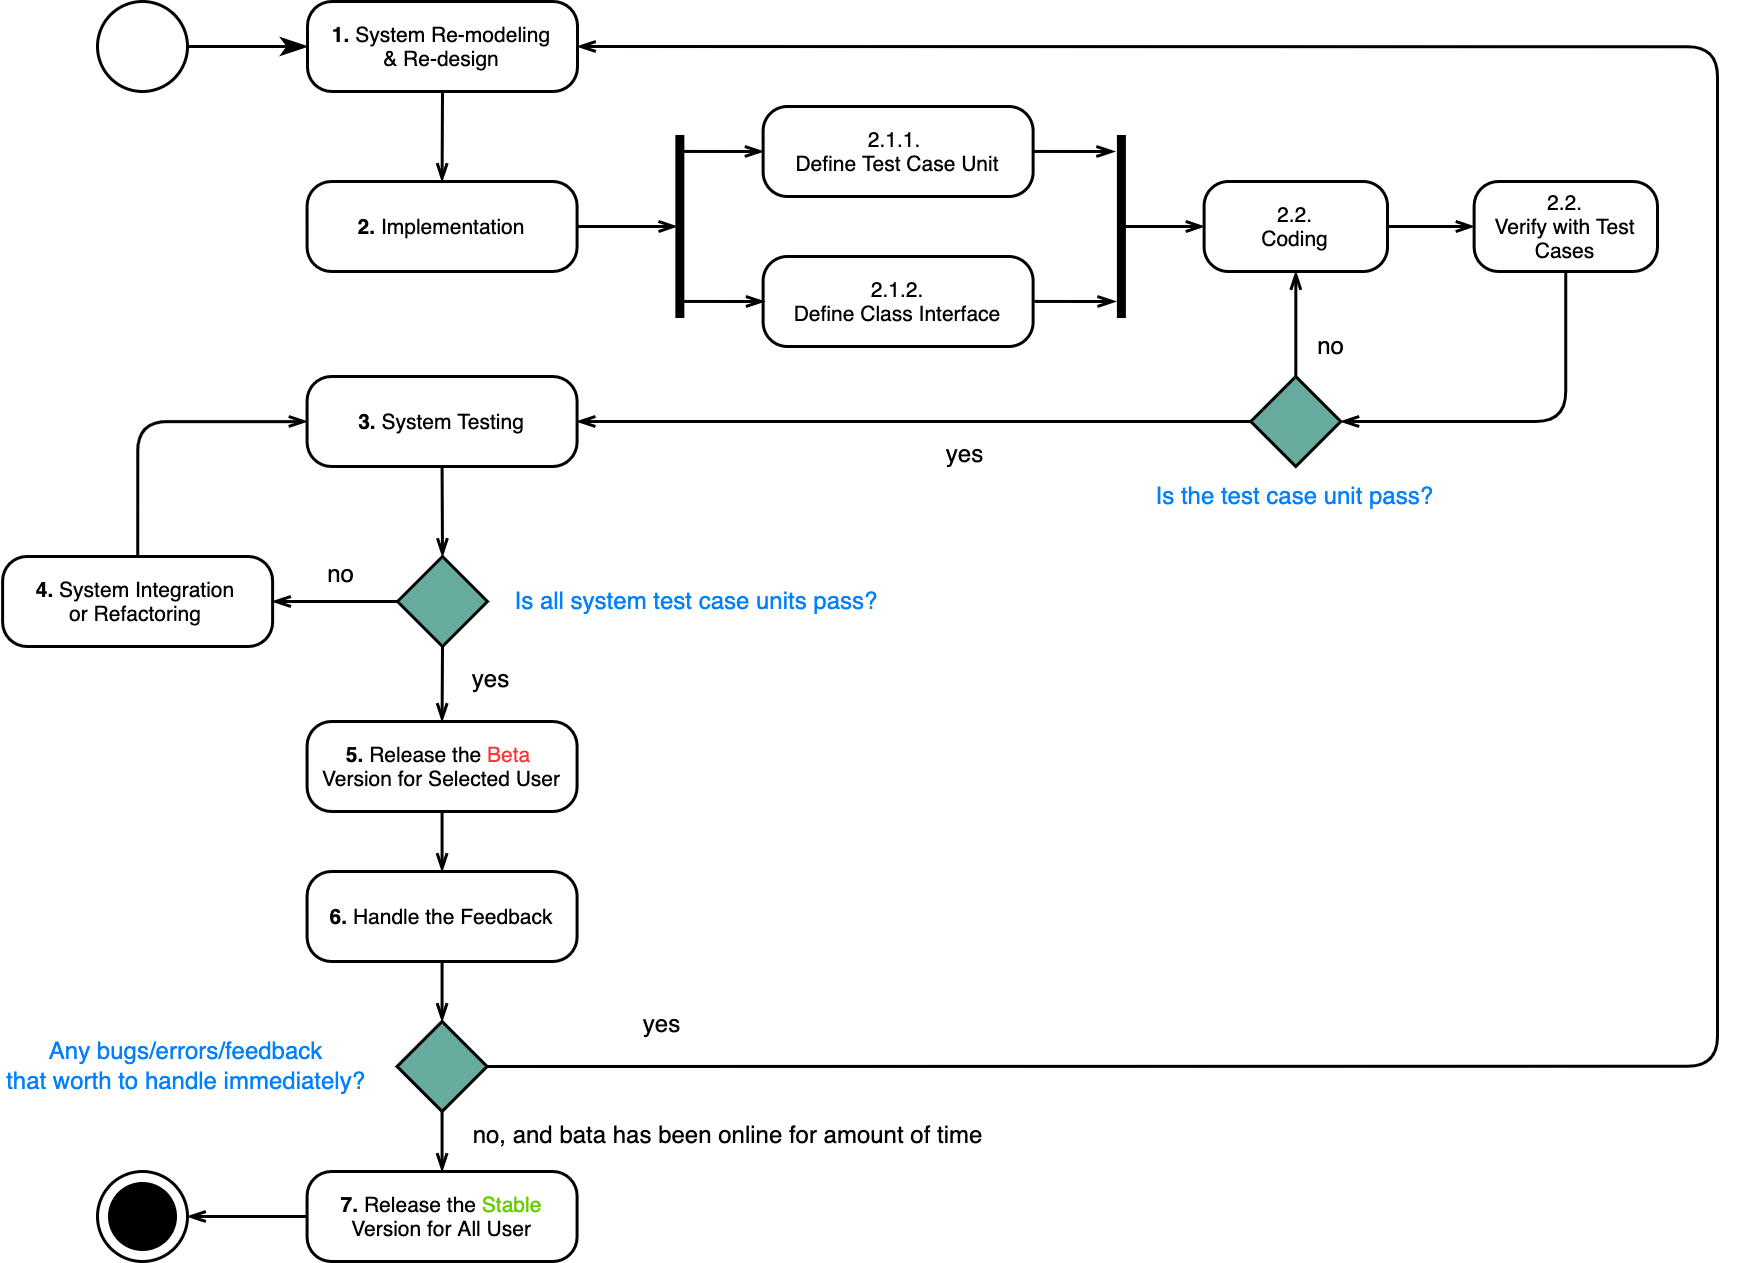
\includegraphics[width=0.9\textwidth]{./img/change-handling-process.png}
	\caption{Activity Diagram of Requirement Change Handling Process}
	\label{fig:incre-process}
\end{figure*}

\section{T2: Context View Modeling 1}

\textit{\textquote{Our solution would
		implement a GPS tracking device accelerometer and gyroscopic sensors to detect
		relevant changes in the state of a parked bike and immediately notify users.}}

As already been presented at the submission of assignment 1,
the external architecture of the system can be seen as a way of the context of the system.
Then it can be described by context model as is shown in Fig \ref{fig:sys-context-model}.

A total of three context objects is involved in this product:

\begin{itemize}
	\item [1.] \textbf{Chip System}: an integrated chip that include all the hareware components.
	      This chip is installed on the bike of users. The chip shall have the ability to communicate with a network endpoint.
	\item [2.] \textbf{Back-end System}: the back-end system wich receive and response a network request send from chips or users' mobile application.
	      Meanwhile, the server can also store the data send from chips.
	\item [3.] \textbf{Mobile Application}: the companion application installed on users' mobile devices.
	      This application can communicate with the back-end server and display all information to the user.
	      Also, users can send instructions to the chips through this application.
\end{itemize}

\begin{figure*}[!ht]
	\centering
	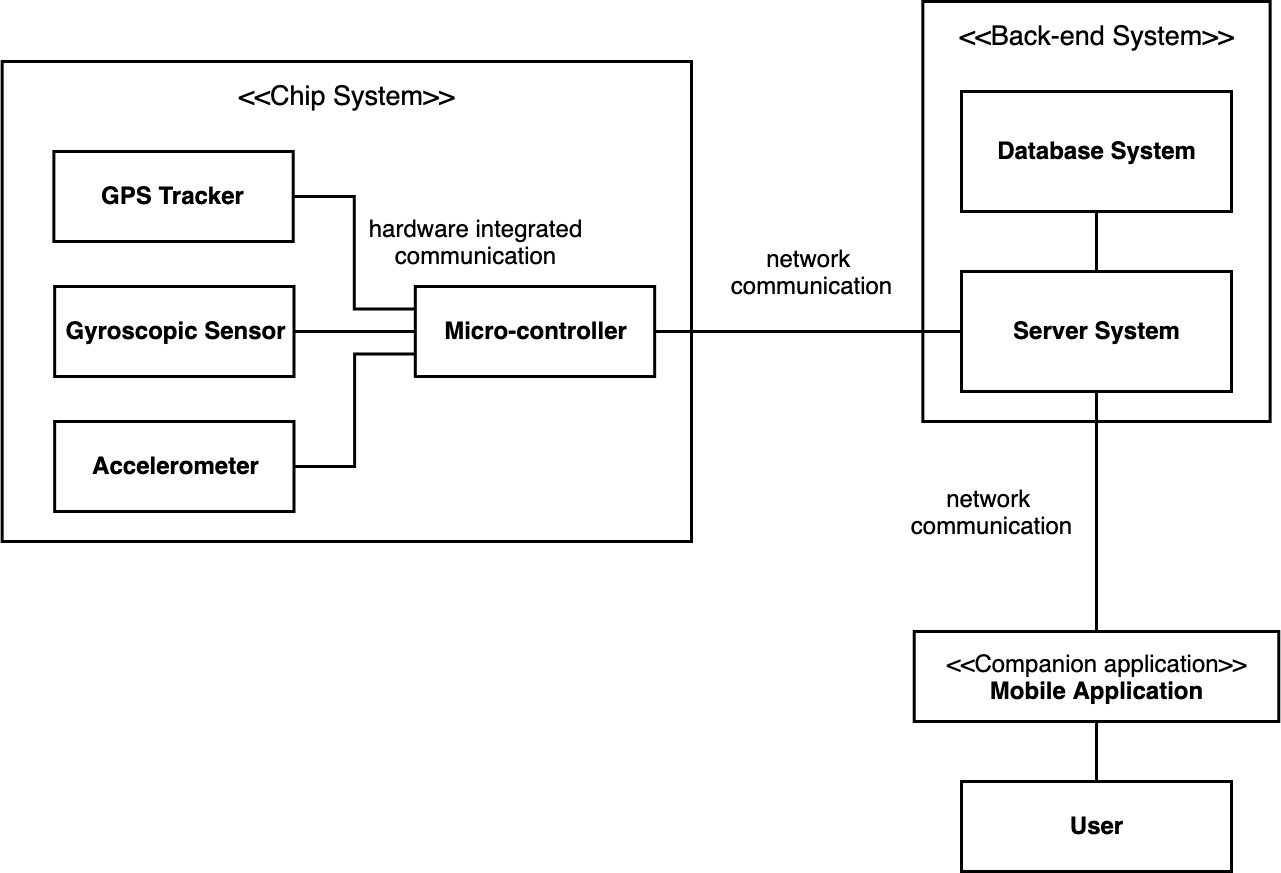
\includegraphics[width=0.7\textwidth]{./img/sys-context-model.png}
	\caption{Block Diagram of System Context of Communication}
	\label{fig:sys-context-model}
\end{figure*}

\section{T3: Context View Modeling 2}

\textit{\textquote{In addition to above
		description, history of the bike tracking can be queried by the user given a time
		span specified by the user. The history is kept maximum for a year. The user can
		choose the time interval between 1 minute, 5 minutes, to 1 hour to record the GPS
		locations of the bike.}}

Fig. \ref{fig:sys-context-model-2}\footnote{Since the chip system is not directly involved in this description, it will not be presented in this diagram.} present the context modeling of the above description.
The explanation dataflow in the diagram are listed below:

\begin{figure}[!ht]
	\centering
	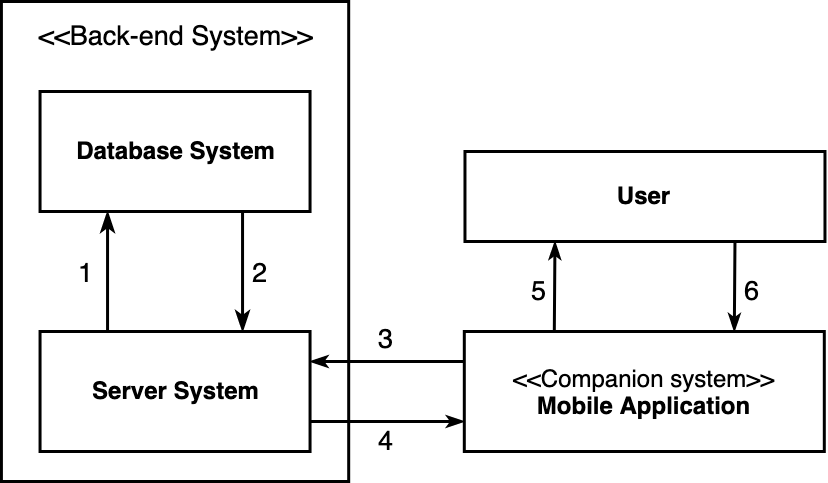
\includegraphics[width=0.45\textwidth]{./img/sys-context-model-2.png}
	\caption{Block Diagram of System Context of History Data Query}
	\label{fig:sys-context-model-2}
\end{figure}

\begin{itemize}
	\item [1.] The back-end server is quering data from the database system.
	\item [2.] The database system is returning data to the back-end system.
	\item [3.] The companion application transfer user's instructions to the back-end system.
	\item [4.] The back-end system response the demanded data to the companion application.
	\item [6.] The user select the time interval on the companion application.
	\item [5.] The companion application display the result to the user.
\end{itemize}

As the product has a back-end server of its own design at the very first place, no new context or stakeholder will be introduced into the product.
Since this new requirement can be handled with a set of new features introduced to the software of the back-end server and the mobile applications.

\begin{figure*}[!ht]
	\centering
	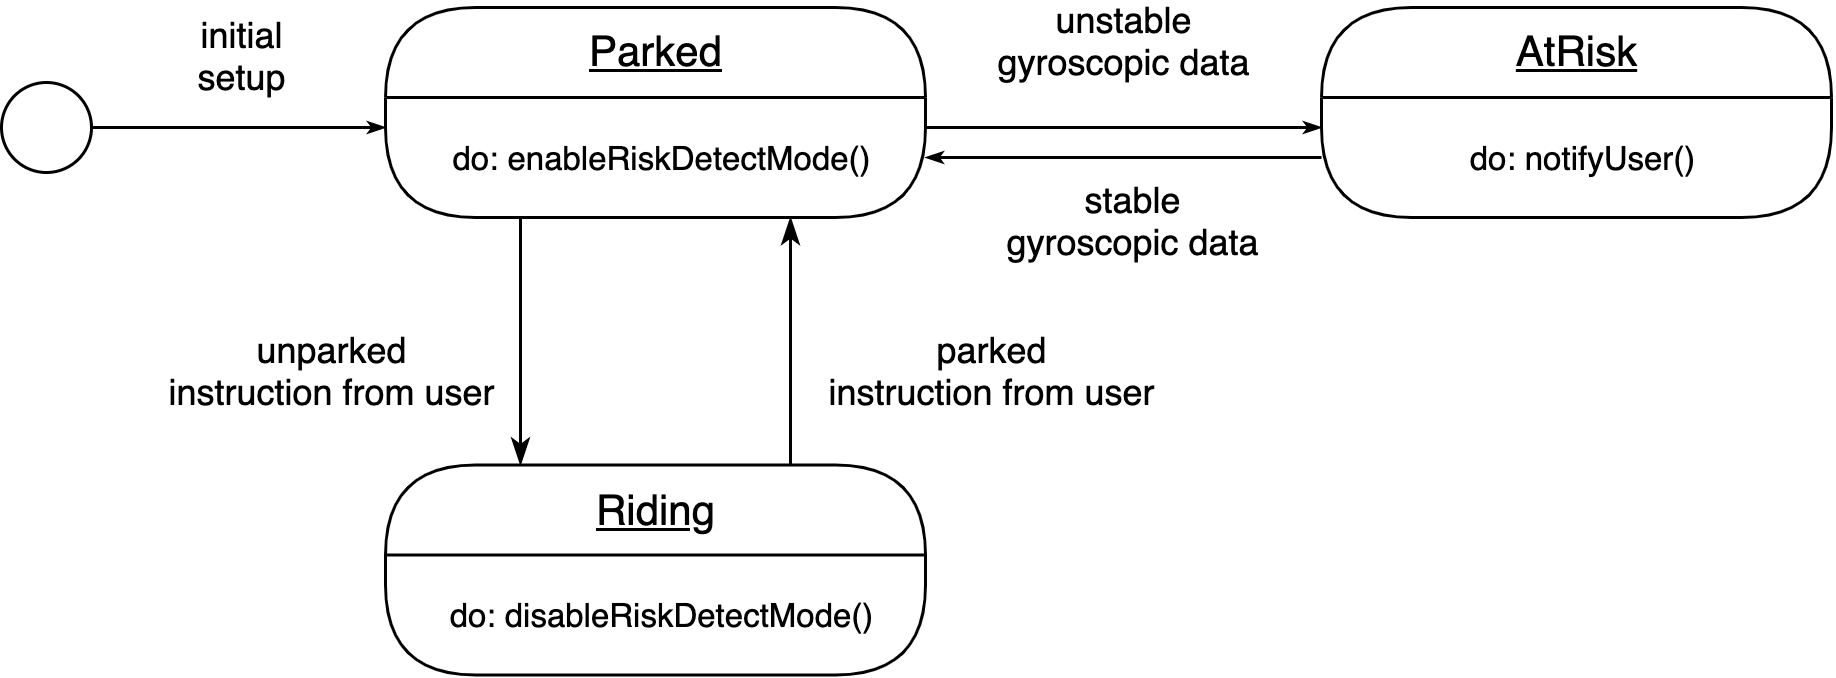
\includegraphics[width=0.8\textwidth]{./img/state-diagram.png}
	\caption{State Diagram of the Chip System}
	\label{fig:state-diagram}
\end{figure*}

\section{T4: Behavioral View Modeling}

\textquote{\textit{The companion application will notify users of these changes
		through push notifications. The application will allow users to track their bike in
		the event immediate intervention is not possible.}}

Fig. \ref{fig:state-diagram} models the above description with an event-driven state diagram.
The diagram represents the state of the chip system. Every chip will switch between those three states that are described below:

\begin{itemize}
	\item [1.] \textbf{\textquote{Parked} State}: the initial state when the user first installs the chip and initialized the chip and the companion application.
	      Users can send an instruction to set this state back to the chip when the previous state is \textquote{Riding} state;
	      Also the \textquote{AtRisk} state can be swith to this state when the gyroscopic data become stable.
	      When the chips are at this state, the chips will automatically exam the gyroscopic data to estimate whether the chip is at the risk of stealing.
	\item [2.] \textbf{\textquote{Riding} State}: the state that represents the bike was being used by the user.
	      Users can inform the chip switch from the \textquote{Parked} state to this state.
	      When the chips are at this state, the chips will not exam the gyroscopic data.
	\item [3.] \textbf{\textquote{AtRisk} State}: the state that can be changed when recieving the unstable gyroscopic data are detected.
	      When the chips are at this state, the chips will send notification to users' companion application.
\end{itemize}

\section{T5: Observer-Subject Design Pattern Implementation}

\textquote{\textit{The companion application will notify users of these changes through
		push notifications. The application will allow users to track their bike in the event
		immediate intervention is not possible.}}

The modelling Class Diagram of applying the observer-subject design pattern to this scenario is shown in Fig. \ref{fig:osp}.
This pattern is used at the back-end server context.

As Fig. \ref{fig:osp} illustrates, the back-end server should manage a subject instance,
and every user device should register on this subject as an observer.
When the server receives the chip data from chips, it should notify the companion applications that installed on the users' devices.

\begin{figure*}[!ht]
	\centering
	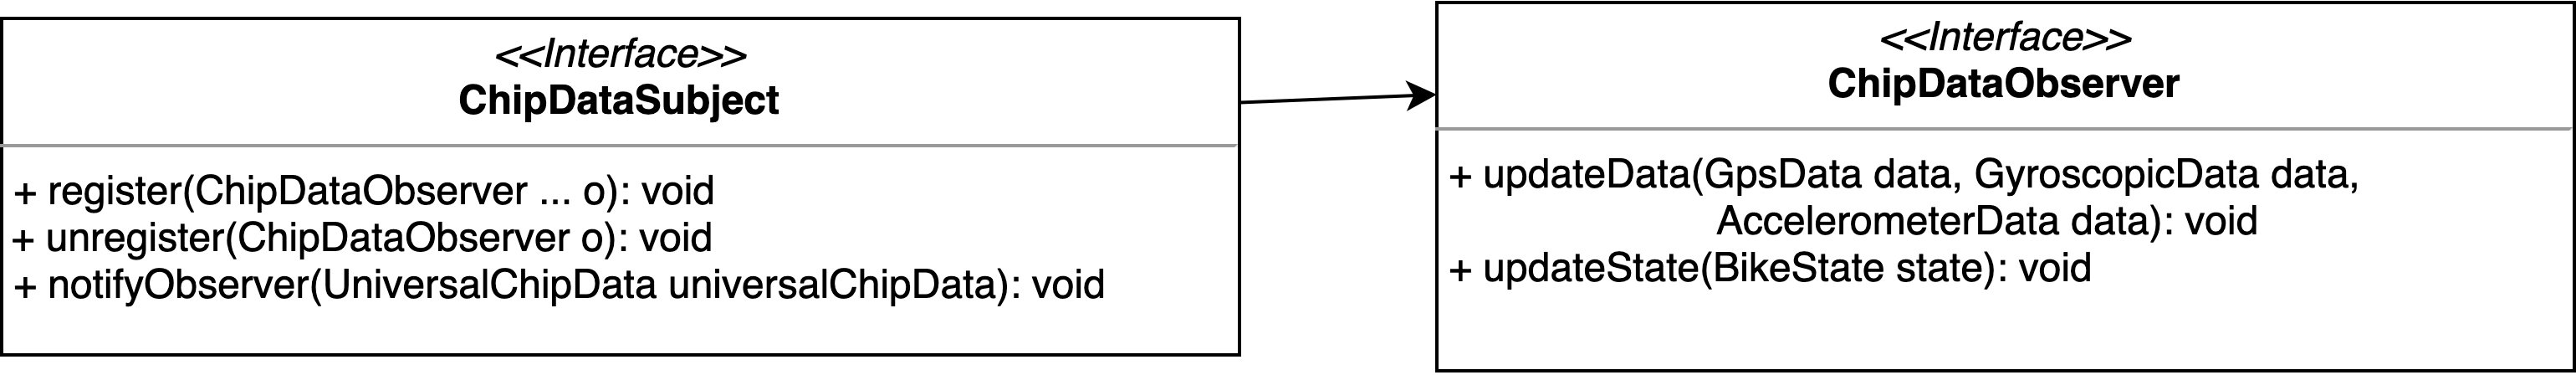
\includegraphics[width=0.9\textwidth]{./img/observer-subject-pattern.png}
	\caption{Class Diagram of the Observer-Subject Design Pattern at the Back-end Server}
	\label{fig:osp}
\end{figure*}

The defined interfaces and the implementation are located at \textquote{/module/communication} package.
The observer implementation is shown in Fig. \ref{fig:observer}.
The subject implementation is shown in Fig. \ref{fig:subject}.

To complete this design pattern, a \textquote{MessageSender} interface that communicates with the users' devices
and a \textquote{RiskDetector} interface that estimates the rick state are defined.

\begin{figure*}[!ht]
	\centering
	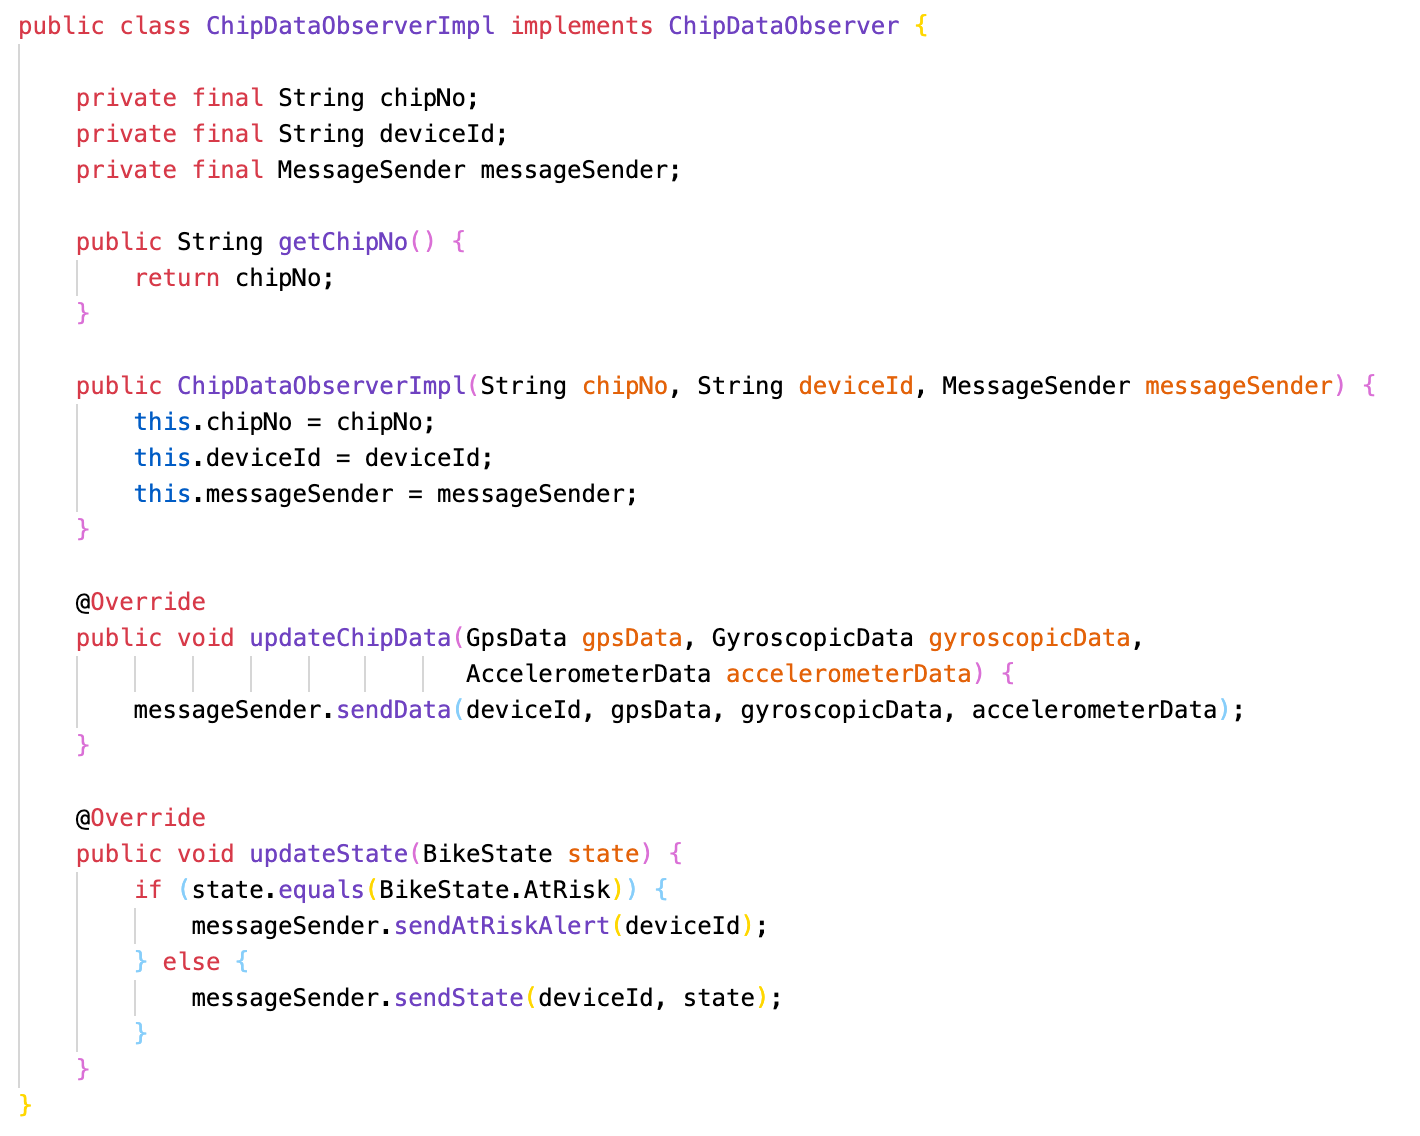
\includegraphics[width=0.9\textwidth]{./img/observer-impl.png}
	\caption{ChipDataObserver Implementation}
	\label{fig:observer}
\end{figure*}

\begin{figure*}[!ht]
	\centering
	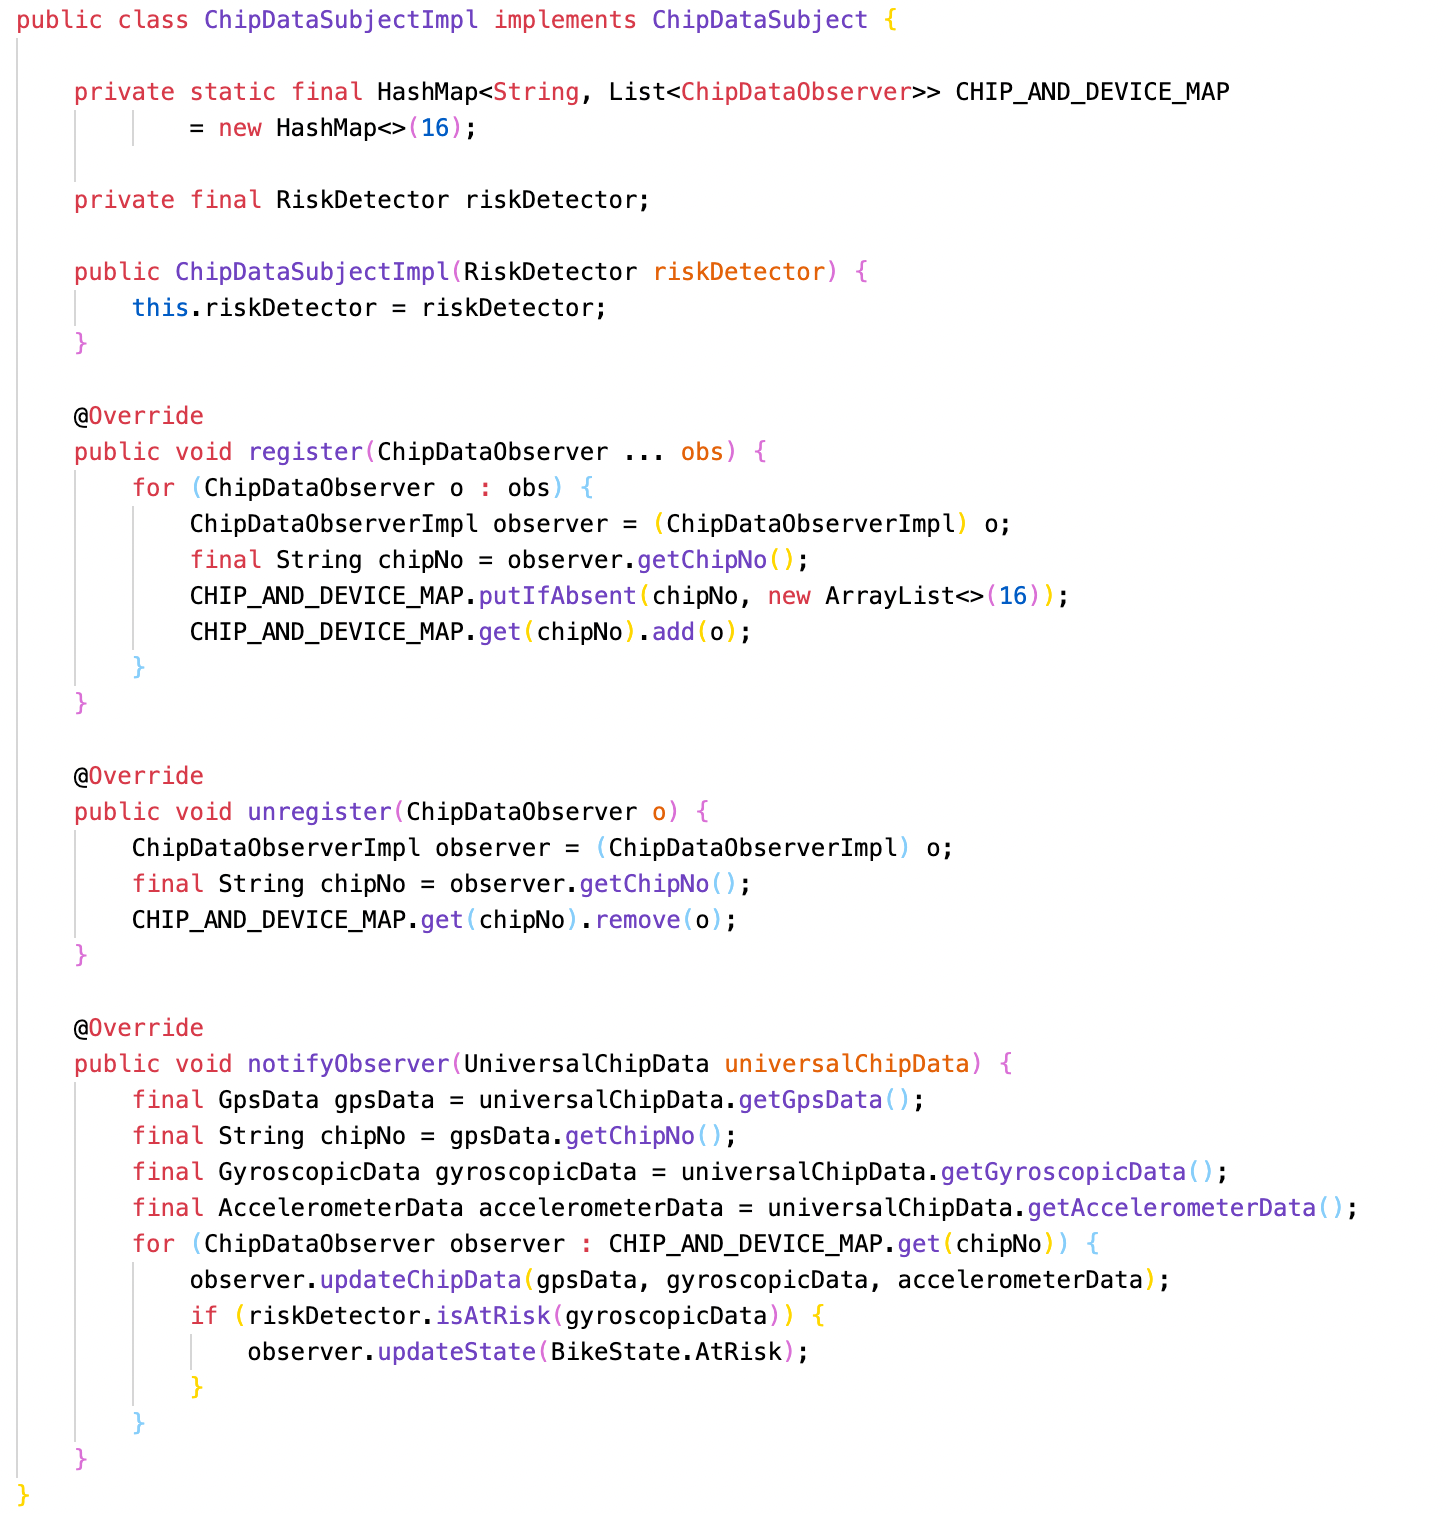
\includegraphics[width=0.9\textwidth]{./img/subject-impl.png}
	\caption{ChipDataSubject Implementation}
	\label{fig:subject}
\end{figure*}

To perform the test cases unit for this design pattern,
the interfaces described above are implemented in test folder as \textquote{MessageSenderTestImpl} and \textquote{RiskDetectorTestImpl}
which are shown in Fig. \ref{fig:messagesender} and Fig. \ref{fig:riskdetector}.

The \textquote{MessageSenderTestImpl} use console printer as a representation of network communication with the users' devices.
And the \textquote{RiskDetectorTestImpl} will estimate risk state by just force the state switch to \textquote{AtRisk} state manually.

The test case unit for all of these interfaces and implementation are presented at \textquotedblleft io/github/youyinnn/module/communication/ChipDataObserverTest.java\textquotedblright .

\begin{figure*}[!ht]
	\centering
	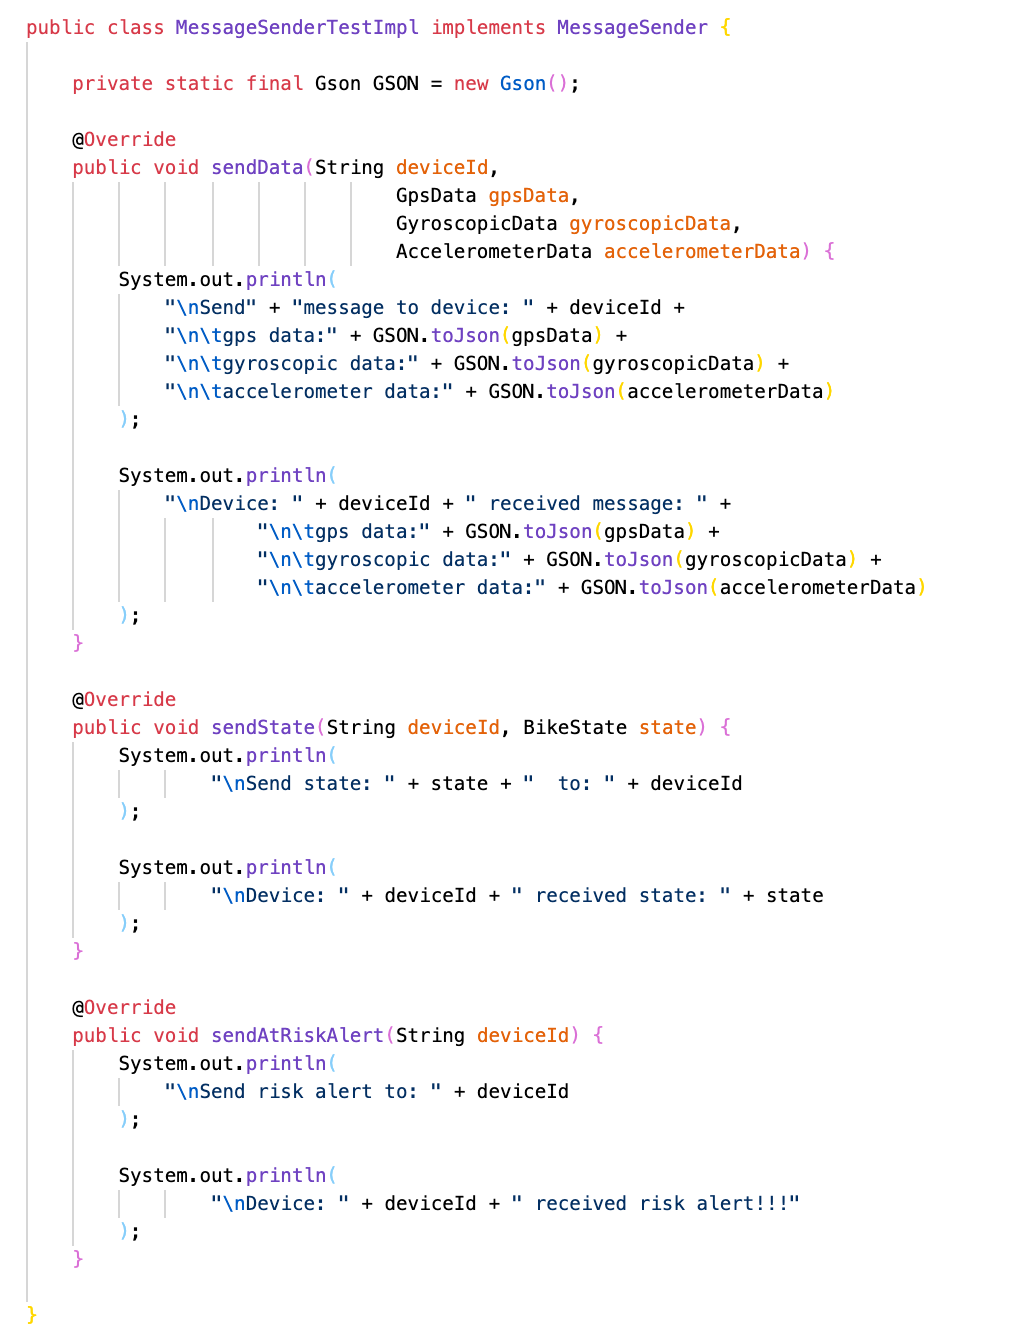
\includegraphics[width=0.8\textwidth]{./img/messagesender.png}
	\caption{MessageSender Testing Implementation}
	\label{fig:messagesender}
\end{figure*}

\begin{figure*}[!ht]
	\centering
	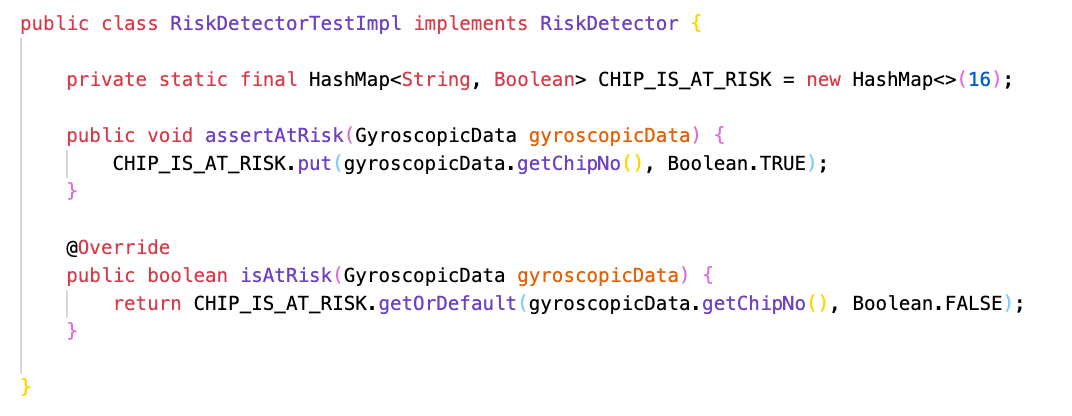
\includegraphics[width=0.8\textwidth]{./img/riskdetector.png}
	\caption{RiskDetector Testing Implementation}
	\label{fig:riskdetector}
\end{figure*}

\end{document}
\endinput